
\de{ĐỀ THI GIỮA HỌC KỲ II NĂM HỌC 2022-2023}{THPT Phạm Phú Thứ}


\begin{bt}%[0T3Y2-1]%[Dự án đề kiểm tra HKII NH22-23- Nguyễn Cường]%[THPT Phạm Phú Thứ]
Dựa vào đồ thị của hàm số bậc hai sau đây, hãy lập bảng xét dấu và kết luận về dấu của tam thức bậc hai tương ứng
\begin{center}
	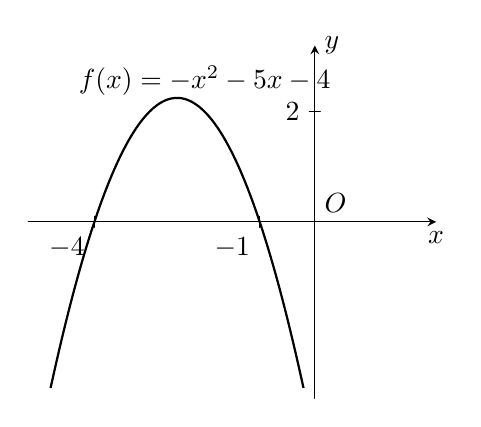
\begin{tikzpicture}[scale=0.7, line join=round, line cap=round, >=stealth]
		\def\xmin{-5}\def\xmax{2}\def\ymin{-3}\def\ymax{3}
		\draw[->] (\xmin-0.2,0)--(\xmax+0.2,0) node[below]{$x$};
		\draw[->] (0,\ymin-0.2)--(0,\ymax+0.2) node[right]{$y$};
		\draw (0,0) node[above right]{$O$};
		\foreach \x in {-4,-1}\draw (\x,0.1)--(\x,-0.1) node[below left]{$\x$};
		\foreach \y in {2}\draw (0.1,\y)--(-0.1,\y) node[left]{$\y$};
		\clip (\xmin,\ymin) rectangle (\xmax,\ymax);
		\draw[thick,smooth,samples=200,domain=\xmin:\xmax] plot (\x,{-1*((\x)^2)+-5*\x+-4});
		\draw (-2,3)node[below]{$f(x)=-x^2-5x-4$};
	\end{tikzpicture}
\end{center}
\loigiai{
Bảng xét dấu của tam thức bậc hai 
\begin{center}

\begin{tikzpicture}[join = round, cap = round, thick, font = \footnotesize, scale = 1]
	\tkzTabInit[lgt=3.5,espcl = 3]
	{$x$ /1, $f(x)$ /1}
	{$-\infty$,$-4$,$-1$,$+\infty$}
	\tkzTabLine{ ,-,z,+,z,-, }
\end{tikzpicture}
\end{center}
Vậy $f(x)>0\Leftrightarrow x\in (-4;-1)$.\\
$f(x)<0\Leftrightarrow x\in (-\infty;-4)\cup (-1;+\infty)$.
}
\end{bt}
\begin{bt}%[0T7B1-1]%[Dự án đề kiểm tra HKII NH22-23- Nguyễn Cường]%[THPT Phạm Phú Thứ]
	Tìm tất cả các giá trị của $m$ để bất phương trình $x^2+(m-2)x-2m+1\ge 0$ nghiệm đúng với mọi $x\in \mathbb{R}$.
	\loigiai{
		Đặt $f(x)=x^2+(m-2)x-2m+1$. Khi đó,
		\allowdisplaybreaks
		\begin{eqnarray*}
			f(x)\ge 0,\,\forall x\in \mathbb{R}&\Leftrightarrow&\heva{&a>0\\&\Delta \le 0}\\
			&\Leftrightarrow&\heva{&1>0\\&(m-2)^2-4(-2m+1)\le 0}\\
			&\Leftrightarrow& m^2+4m\le 0\\
			&\Leftrightarrow& -4\le m\le 0.
		\end{eqnarray*}
Vậy $m\in [-4;0]$.
	}
\end{bt}
\begin{bt}%[0T7B2-1]%[Dự án đề kiểm tra HKII NH22-23- Nguyễn Cường]%[THPT Phạm Phú Thứ]
	Tìm tất cả các giá trị của $m$ để phương trình $(m+2)x^2+mx+m-2=0$ có hai nghiệm phân biệt.
	\loigiai{
	Phương trình có hai nghiệm phân biệt khi và chỉ khi
		\allowdisplaybreaks
		\begin{eqnarray*}
			&&\heva{&a\ne 0\\&\Delta >0}\\
			&\Leftrightarrow&\heva{&m+2\ne 0\\&m^2-4(m+2)(m-2)>0}\\
			&\Leftrightarrow& \heva{&m\ne -2\\&-3m^2+16>0}\\
			&\Leftrightarrow& \heva{&m\ne -2\\&-\dfrac{4\sqrt{3}}{3}<m<\dfrac{4\sqrt{3}}{3}}
		\end{eqnarray*}
		Vậy $m\in \left(-\dfrac{4\sqrt{3}}{3};\dfrac{4\sqrt{3}}{3}\right)\setminus\{-2\}$.
	}
\end{bt}
\begin{bt}%[0T3B2-5]%[Dự án đề kiểm tra HKII NH22-23- Nguyễn Cường]%[THPT Phạm Phú Thứ]
	Độ cao so với mặt đất của một quả bóng được ném lên theo phương thẳng đứng được mô ta bởi hàm số bậc hai $h(t)=-4{,}9t^2+20t+1$, ở đó độ cao $h(t)$ được tính bằng mét và thời gian $t$ được tính bằng giây. Hỏi quả bóng ở độ cao trên $5$ m so với mặt đất trong khoảng thời gian bao lâu? Làm tròn kết quả đến hàng phần trăm.
	\loigiai{
	Ta có $h(t)>5\Leftrightarrow -4{,}9t^2+20t+1> 5\Leftrightarrow -4{,}9t^2+20t-4>0\Leftrightarrow 0{,}21< t<3{,}87$.\\
	Vậy thời gian quả bóng ở độ cao trên $5$ m so với mặt đất trong khoảng $3{,}66$ giây.
	}
\end{bt}

\begin{bt}%[0H9B1-3]%[Dự án đề kiểm tra HKII NH22-23 - Don Lee]%[THPT Phạm Phú Thứ]
	Trong mặt phẳng $Oxy$, cho tam giác $ABC$ có tọa độ các đỉnh là $A(4;3)$, $B(1;3)$, $C(1;-1)$.
	\begin{enumerate}
		\item Chứng minh tam giác $ABC$ vuông. Tính diện tích tam giác $ABC$.
		\item Tìm tọa độ điểm $D$ để $ABCD$ là hình bình hành. Tìm tọa độ tâm hình bình hành $ABCD$.
		\item Tìm tọa độ điểm $H$ là chân đường cao của tam giác $ABC$ kẻ từ $B$.
	\end{enumerate}
	\loigiai{
		\begin{enumerate}
			\item Ta có $\overrightarrow{AB}=(-3;0)$, $\overrightarrow{BC}=(0;-4)$.\\
				Do $\overrightarrow{AB}\cdot \overrightarrow{BC}=-3\cdot 0+0\cdot (-4)=0$ nên $AB\perp BC$, suy ra $\triangle ABC$ vuông tại $B$.\\
				$S_{ABC}=\dfrac{1}{2}\cdot AB\cdot BC=\dfrac{1}{2}\cdot 3\cdot 4=6$.
			\item Ba điểm $A$, $B$, $C$ không thẳng hàng nên $ABCD$ là hình bình hành khi $\overrightarrow{DC}=\overrightarrow{AB}$\\
			$\Leftrightarrow \heva{&1-x_D=-3\\&-1-y_D=0} \Leftrightarrow \heva{&x_D=4\\&y_D=-1.}$\\
			Vậy $D(4;-1)$.
			\item Ta có $\overrightarrow{AC}=(-2;5)$, chọn $\overrightarrow{u}=(-2;5)$ là véc-tơ chỉ phương của đường thẳng $AC$. Phương trình $AC\colon \heva{&x=1-2t\\&y=-2+5t.}$\\
			Gọi $H(1-2t;-2+5t)$ là chân đường cạo kẻ từ $B$ của $\triangle ABC$. Ta có $BH\perp AC$\\
			$\Leftrightarrow \overrightarrow{BH}\cdot \overrightarrow{AC}=0 \Leftrightarrow (-1-2t)\cdot (-2)+(-2+5t)\cdot 5=0 \Leftrightarrow t=\dfrac{8}{29}$.\\
			Vậy $H\left(\dfrac{13}{29}; -\dfrac{18}{29}\right)$.
		\end{enumerate}
	}
\end{bt}

\begin{bt}%[0H9B2-2]%[Dự án đề kiểm tra HKII NH22-23 - Don Lee]%[THPT Phạm Phú Thứ]
	Trong mặt phẳng $Oxy$, cho tam giác $ABC$ có tọa độ các đỉnh là $A(1;2)$, $B(2;0)$, $C(-1;3)$.
	\begin{enumerate}
		\item Viết phương trình đường thẳng $AB$.
		\item Viết phương trình đường trung trực $\Delta$ của cạnh $AC$.
	\end{enumerate}
	\loigiai{
		\begin{enumerate}
			\item Ta có $\overrightarrow{AB}=(1;-2)$, chọn $\overrightarrow{n}=(2;1)$ là véc-tơ pháp tuyến của $AB$.\\
			Phương trình $AB\colon 2\cdot(x-2)+1\cdot(y-0)=0 \Leftrightarrow 2x+y-4=0$.
			\item Ta có $\overrightarrow{AC}=(-2;1)$ và $I\left(0;\dfrac{5}{2}\right)$ là trung điểm $AC$.\\
			Đường thẳng $\Delta$ đi qua $I$ và nhận $\overrightarrow{n}_{1}=(2;-1)$ là véc-tơ pháp tuyến nên có phương trình
			\[2\cdot (x-0)-1\cdot\left(y-\dfrac{5}{2}\right)=0 \Leftrightarrow 2x-y+\dfrac{5}{2}=0 \Leftrightarrow 4x-2y+5=0.\]
		\end{enumerate}
	}
\end{bt}

\begin{bt}%[0H9B2-6]%[Dự án đề kiểm tra HKII NH22-23 - Don Lee]%[THPT Phạm Phú Thứ]
	Trong mặt phẳng $Oxy$, cho hai điểm $A(4;-2)$, $B(10;4)$. Tìm tọa độ điểm $M$ thuộc trục hoành sao cho $\left|\overrightarrow{MA}+\overrightarrow{MB}\right|$ nhỏ nhất.
	\loigiai{
		Gọi $I(7;1)$ là trung điểm của $AB$.\\
		Ta có $P=\left|\overrightarrow{MA}+\overrightarrow{MB}\right|=2\left|\overrightarrow{MI}\right|=2IM$.\\
		Do đó $P_{\min}$ khi $IM_{\min}$ khi $M$ là hình chiếu của $I$ trên $Ox$. Suy ra $M(7;0)$.
	}
\end{bt}










